\documentclass[a4paper, 11pt]{article}

%Comandos para configurar el idioma
\usepackage[spanish,activeacute]{babel}
\usepackage[utf8]{inputenc}
\usepackage[T1]{fontenc} %Necesario para el uso de las comillas latinas.
\usepackage{geometry}
\usepackage{graphicx}

%Importante que esta sea la última órden del preámbulo
\usepackage{hyperref}

\newcommand\fnurl[2]{%
  \href{#2}{#1}\footnote{\url{#2}}%
}

\newcommand{\includecode}[2][c]{\lstinputlisting[caption=#2, escapechar=, style=custom#1]{#2}<!---->}

%Paquetes matemáticos
\usepackage{amsmath,amsfonts,amsthm}
\usepackage[all]{xy} %Para diagramas
\usepackage{enumerate} %Personalización de enumeraciones
\usepackage{tikz} %Dibujos

%Tipografía escalable
\usepackage{lmodern}
%Legibilidad
\usepackage{microtype}

%Código
\usepackage{listings}
\usepackage{color}

\definecolor{dkgreen}{rgb}{0,0.6,0}
\definecolor{gray}{rgb}{0.5,0.5,0.5}
\definecolor{mauve}{rgb}{0.58,0,0.82}

\definecolor{listinggray}{gray}{0.9}
\definecolor{lbcolor}{rgb}{0.9,0.9,0.9}
\lstset{
backgroundcolor=\color{lbcolor},
    tabsize=4,
rulecolor=,
    language=[GNU]C++,
        basicstyle=\scriptsize,
        upquote=true,
        aboveskip={1.5\baselineskip},
        columns=fixed,
        showstringspaces=false,
        extendedchars=false,
        breaklines=true,
        prebreak = \raisebox{0ex}[0ex][0ex]{\ensuremath{\hookleftarrow}},
        frame=single,
        numbers=left,
        showtabs=false,
        showspaces=false,
        showstringspaces=false,
        identifierstyle=\ttfamily,
        keywordstyle=\color[rgb]{0,0,1},
        commentstyle=\color[rgb]{0.026,0.112,0.095},
        stringstyle=\color[rgb]{0.627,0.126,0.941},
        numberstyle=\color[rgb]{0.205, 0.142, 0.73},
%        \lstdefinestyle{C++}{language=C++,style=numbers}’.
}
\lstset{
    backgroundcolor=\color{lbcolor},
    tabsize=4,
  language=C++,
  captionpos=b,
  tabsize=3,
  frame=lines,
  numbers=left,
  numberstyle=\tiny,
  numbersep=5pt,
  breaklines=true,
  showstringspaces=false,
  basicstyle=\footnotesize,
%  identifierstyle=\color{magenta},
  keywordstyle=\color[rgb]{0,0,1},
  commentstyle=\color[rgb]{0.026,0.112,0.095}, % Darkgreen
  stringstyle=\color{red}
  }
% Slightly bigger margins than the latex defaults

\geometry{verbose,tmargin=1in,bmargin=1in,lmargin=1in,rmargin=1in}
\setlength{\parskip}{.5em} % por defecto el espacio entre párrafos es 0pt

\theoremstyle{definition}
\newtheorem{ejercicio}{Ejercicio}
\newtheorem{cuestion}{Cuestión}
\newtheorem*{solucion}{Solución}
\newtheorem*{bonus}{BONUS}

%%%%%%%% New sqrt
\usepackage{letltxmacro}
\makeatletter
\let\oldr@@t\r@@t
\def\r@@t#1#2{%
\setbox0=\hbox{$\oldr@@t#1{#2\,}$}\dimen0=\ht0
\advance\dimen0-0.2\ht0
\setbox2=\hbox{\vrule height\ht0 depth -\dimen0}%
{\box0\lower0.4pt\box2}}
\LetLtxMacro{\oldsqrt}{\sqrt}
\renewcommand*{\sqrt}[2][\ ]{\oldsqrt[#1]{#2} }
\makeatother

%%%%%%%%%%%%%%%%%%%%%%%%%%%%%%%%%%%%%%%%%%%

\hypersetup{
  pdftitle={Informe de trabajo 3},
  pdfauthor={Antonio Álvarez Caballero},
  unicode,
  breaklinks=true,  % so long urls are correctly broken across lines
  colorlinks=true,
  urlcolor=blue,
  linkcolor=blue,
  citecolor=darkgreen,
  }

\title{Informe de trabajo 3}
\author{Antonio Álvarez Caballero\\
    \href{mailto:analca3@correo.ugr.es}{analca3@correo.ugr.es}}
\date{}
%%%%%%%%%%%%%%%%% FIN PREAMBULO %%%%%%%%%%%%%%%%%%%%%%%%%%%

\begin{document}

  \maketitle

  \section{Estimación de una cámara a partir del conjunto de puntos en correspondencias}

    La primera parte de la práctica consiste en estimar una cámara finita a partir de un
    conjunto de puntos en correspondencias.

    \subsection{Cámara finita aleatoria}

      Primero debemos generar una cámara finita $P$ a partir de valores aleatorios en $[0,1]$.
      Para ello usaremos el propio generador de números de \emph{OpenCV}. Para ello primero
      debemos asignar su estado al reloj actual (para asegurar aleatoriedad) y después
      usaremos la función \emph{randu}, que devuelve una matriz aleatoria con valores
      entre los valores de entrada uniformemente distribuidos. Nos la quedamos si y solamente si
      es finita, lo cual significa que la submatriz $3\times3$ principal es regular.

      \begin{lstlisting}
        theRNG().state = clock();
        ...

        bool Camera::isFinite()
        {
          // Check if the first 3x3 submatrix is regular
          Mat M = this->camera(Rect(0,0,3,3));
          return determinant(M) != 0.0;
        }

        Camera::Camera(float low, float high)
        {
          // Fill 3x4 matrix with zeros
          this->camera = Mat::zeros(3, 4, CV_32FC1);

          while (!this->isFinite())
          {
            // Set this->camera to randon matrix. Random values are uniformly distributed from low to high
            randu(this->camera,low,high);
          }
        }
      \end{lstlisting}

    \subsection{Simular patrón de puntos y proyectar}

      Ahora suponemos el patrón de puntos indicado y los proyectamos usando nuestra
      cámara finita. Esto es simplemente tomando coordenadas homogéneas y multiplicando
      matriz por punto. Después homogeneizamos la salida y tomamos sólo las componentes $X$ e $Y$.


      \begin{lstlisting}
        Point2f Camera::project(Point3f input)
        {
          // Take input with homogeneous coordinates
          Vec4f homogeneous (input.x, input.y, input.z, 1.0);

          // Product with the camera
          Mat result = this->camera * Mat(homogeneous);

          // Quotient two first coordinates with last one
          Point2f projection (result.at<float>(0) / result.at<float>(2), result.at<float>(1) / result.at<float>(2));

          return projection;

        }
      \end{lstlisting}

      \subsection{Estimación de la cámara con correspondencias}
      Ahora estamos en condiciones de estimar una cámara con los puntos 3D del mundo y
      sus proyecciones en la imagen. Para ello usaremos el algoritmo DLT. Debemos resolver
      un sistema de ecuaciones de la misma manera que en la anterior práctica (Haciendo \emph{SVD} y tomando la fila asociada al valor singular más pequeño).

      La matriz del sistema está corregida en Hartley \& Ziselmann.

      \begin{lstlisting}
        Camera::Camera(vector< pair<Point3f, Point2f> > correspondences)
        {
          this->camera = Mat::zeros(3, 4, CV_32FC1);
          Mat A = Mat::zeros(2 * correspondences.size(), 12, CV_32FC1);

          for (unsigned i = 0; i < correspondences.size(); i++)
          {
            A.at<float>(2 * i, 4) = -correspondences[i].first.x;
            A.at<float>(2 * i, 5) = -correspondences[i].first.y;
            A.at<float>(2 * i, 6) = -correspondences[i].first.z;
            A.at<float>(2 * i, 7) = -1.0;
            A.at<float>(2 * i, 8) = correspondences[i].second.y * correspondences[i].first.x;
            A.at<float>(2 * i, 9) = correspondences[i].second.y * correspondences[i].first.y;
            A.at<float>(2 * i,10) = correspondences[i].second.y * correspondences[i].first.z;
            A.at<float>(2 * i,11) = correspondences[i].second.y;

            A.at<float>(2 * i + 1, 0) = correspondences[i].first.x;
            A.at<float>(2 * i + 1, 1) = correspondences[i].first.y;
            A.at<float>(2 * i + 1, 2) = correspondences[i].first.z;
            A.at<float>(2 * i + 1, 3) = 1.0;
            A.at<float>(2 * i + 1, 8) = -correspondences[i].second.x * correspondences[i].first.x;
            A.at<float>(2 * i + 1, 9) = -correspondences[i].second.x * correspondences[i].first.y;
            A.at<float>(2 * i + 1,10) = -correspondences[i].second.x * correspondences[i].first.z;
            A.at<float>(2 * i + 1,11) = -correspondences[i].second.x;
          }

          Mat w, u ,vt;
          SVD::compute(A, w, u, vt);

          for (int i = 0; i < 3; i++)
        		for (int j = 0; j < 4; j++)
        			this->camera.at<float>(i, j) = vt.at<float>(11, i * 4 + j);
        }

      \end{lstlisting}

      Ahora, para valorar la estimación, calcularemos el error de la cámara estimada con
      respecto a la simulada. Se usa la \emph{Norma de Frobenius cuadrática}.

      \begin{lstlisting}
        float Camera::error(Camera other)
        {
          Mat one = this->camera / this->camera.at<float>(2,2);
          Mat two = other.camera / other.camera.at<float>(2,2);

          Mat diff = one - two;
          float error = 0.0;

          for (int i = 0; i < diff.rows; i++)
            for (int j = 0; j < diff.cols; j++)
              error += diff.at<float>(i,j) * diff.at<float>(i,j);

          return error;
        }
      \end{lstlisting}

      En nuestro caso obtenemos un error de $2.14488 \times 10^{-10}$, lo cual nos muestra
      que la estimación es muy buena. Prueba de ello es que los puntos se solapan en la imagen.
      Los puntos están escalados para que no queden todos en la esquina superior izquierda. \\

      \centerline{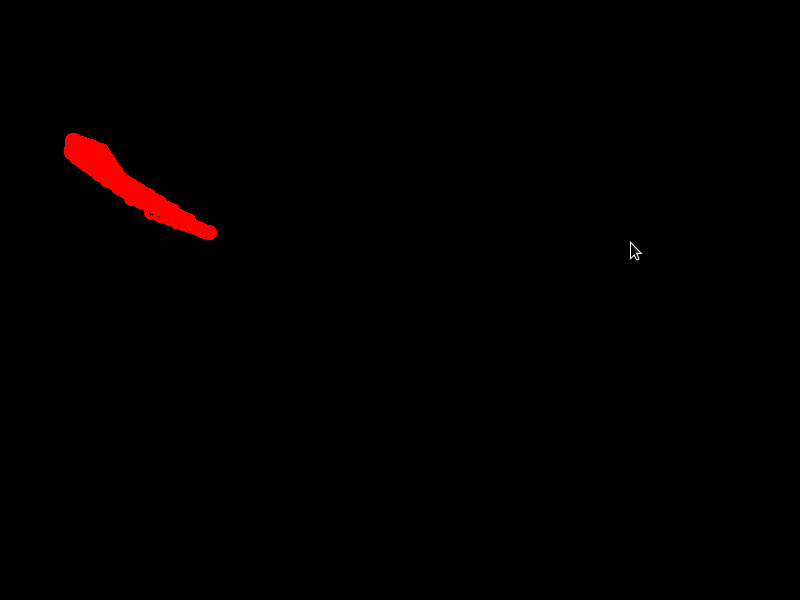
\includegraphics[width=0.7\textwidth]{CamaraSimulada.png}}

    \section{Calibración de cámara usando homografías}

      El próximo punto de la práctica es calibrar una cámara usando homografías.
      Para ello buscaremos las esquinas interiores de un tablero similar al de ajedrez aunque más grande.

      \subsection{Buscando esquinas}
        El primer paso es buscar las esquinas interiores del tablero usando \emph{findChessboardCorners()}.
        Una vez las tengamos, si forman el patrón deseado (en nuestro caso $13\times12$) refinaremos sus coordenadas
        e iremos añadiendo dichas imágenes a lo que hemos llamado \emph{imágenes válidas}.

        El tamaño de la ventana de cornerSubPix lo dejamos en lo que se podría llamar por defecto,
        ya que en muchos ejemplos (tanto de la red como de la propia documentación de \emph{OpenCV})
        se deja en \emph{Size(5,5)}, y el tamaño zero o zona muerta lo dejamos a cero, \emph{Size(-1,-1)}.

      \begin{lstlisting}
        const int CHESS_IMAGES = 25;
        bool valid;
        vector<Point2f> corners;
        vector< vector<Point2f> > imagePoints;
        vector<Mat> images(CHESS_IMAGES);
        vector<Mat> valid_images;
        Size patternSize(13,12);

        for (int i = 0; i < CHESS_IMAGES; i++)
        {
          images[i] = imread("imagenes/Image" + to_string(i+1) + ".tif", CV_LOAD_IMAGE_GRAYSCALE);
          valid = cv::findChessboardCorners(images[i], patternSize, corners);

          if (valid)
          {
            cornerSubPix(images[i], corners, Size(5, 5), Size(-1, -1),
              TermCriteria());
            valid_images.push_back(images[i]);
            imagePoints.push_back(corners);
            cv::drawChessboardCorners(images[i], patternSize, corners, valid);
          }
        }
      \end{lstlisting}

      En nuestro caso se toman $4$ imágenes como válidas, ya que se detecta el patrón, y se muestran
      por pantalla. \\

      \centerline{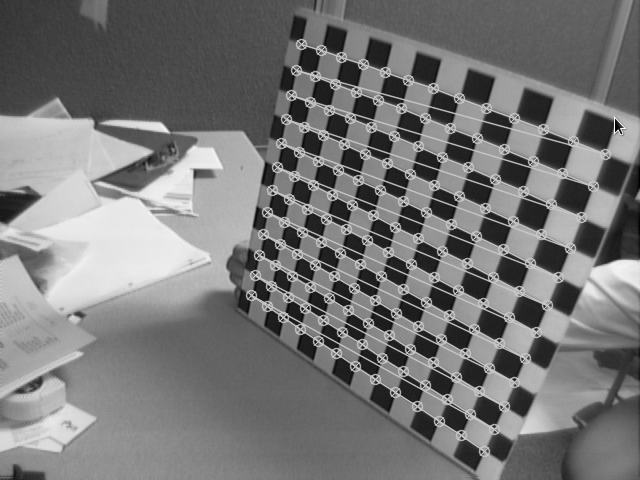
\includegraphics[width=0.7\textwidth]{Tablero1.png}}
      \centerline{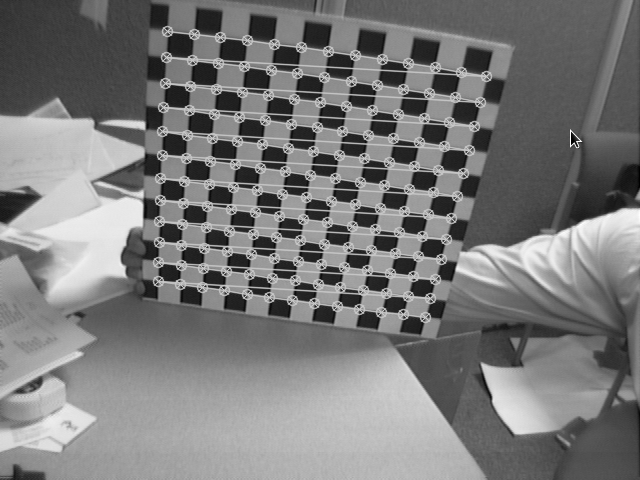
\includegraphics[width=0.7\textwidth]{Tablero2.png}}
      \centerline{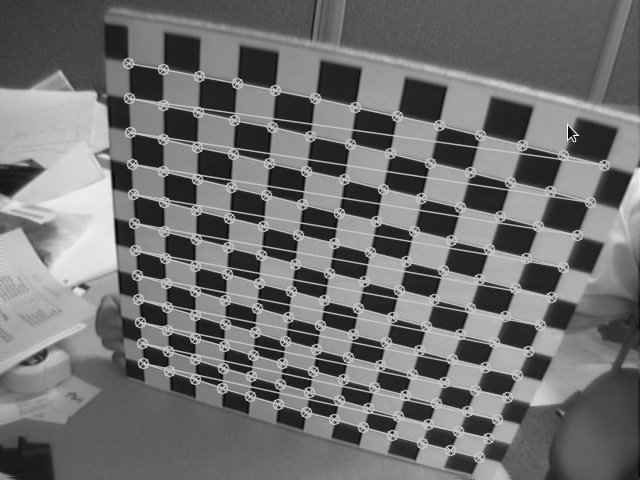
\includegraphics[width=0.7\textwidth]{Tablero3.png}}
      \centerline{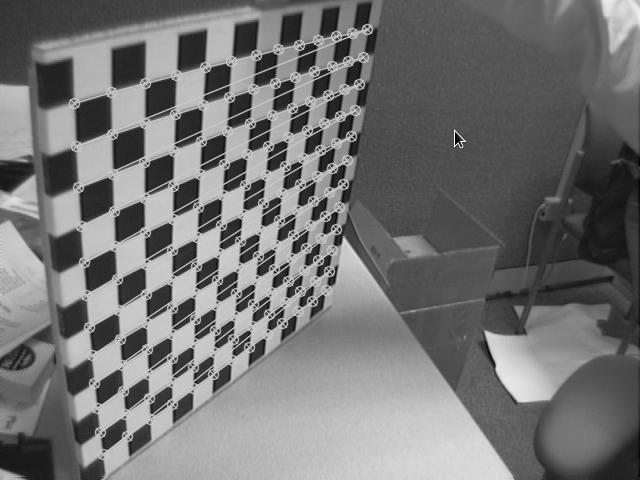
\includegraphics[width=0.7\textwidth]{Tablero4.png}}

      \subsection{Calibración de la cámara}

      Ahora con los datos obtenidos debemos conseguir una matriz cámara con la función
      \emph{calibrateCamera}. Nuestros \emph{objectPoints} son una numeración de las esquinas del tablero.

      Los flags de distorsión vienen en la documentación, se ha calibrado la cámara
      en 4 supuestos: sin distorsión, distorsión radial, distorsión tangencial y
      todas las distorsiones.

      \begin{lstlisting}
        vector< vector<Point3f> > objectPoints;
        vector<Point3f> points;
        for (int i = 0; i < 12; i++) {
          for (int j = 0; j < 13; j++) {
            Point3f p = Point3f(j,i,0);
            points.push_back(p);
          }
        }

        for (unsigned i = 0; i < valid_images.size(); i++)
        {
          objectPoints.push_back(points);
        }

        Mat cameraMatrix = Mat(3, 3, CV_32F);
        Size imageSize(valid_images[0].cols, valid_images[0].rows);
        Mat distCoeffs = Mat(8, 1, CV_32F);
        vector< Mat > rotationVectors;
        vector< Mat > translationVectors;

        int no_distorsion_flags = CV_CALIB_ZERO_TANGENT_DIST | CV_CALIB_FIX_K1 | CV_CALIB_FIX_K2 | CV_CALIB_FIX_K3;
        int radial_distorsion_flags = CV_CALIB_ZERO_TANGENT_DIST;
        int tangential_distorsion_flags = CV_CALIB_FIX_K1 | CV_CALIB_FIX_K2 | CV_CALIB_FIX_K3;

        double error_no_distorsion = calibrateCamera(objectPoints, imagePoints, imageSize, cameraMatrix, distCoeffs, rotationVectors, translationVectors, no_distorsion_flags);
        double error_radial_distorsion = calibrateCamera(objectPoints, imagePoints, imageSize, cameraMatrix, distCoeffs, rotationVectors, translationVectors, radial_distorsion_flags);
        double error_tangential_distorsion = calibrateCamera(objectPoints, imagePoints, imageSize, cameraMatrix, distCoeffs, rotationVectors, translationVectors, tangential_distorsion_flags);
        double error_all_distorsion = calibrateCamera(objectPoints, imagePoints, imageSize, cameraMatrix, distCoeffs, rotationVectors, translationVectors, 0);

      \end{lstlisting}

      Los resultados son estos:

      Error calibrando sin distorsión = 1.3254 \\
      Error calibrando con distorsión radial = 0.163034 \\
      Error calibrando con distorsión tangencial = 1.30143 \\
      Error calibrando con todas las distorsiones = 0.162133 \\

      La distorsión tangencial no afecta tanto en esta cámara como la radial, como se puede
      ver en los errores que introduce cada una de ellas.

  \section{Estimación de la matriz fundamental}

    En esta parte de la práctica tenemos que, usando el detector \emph{BRISK},
    detectar las regiones relevantes de las imágenes de \emph{Vmort} $1$ y $2$.
    Además tenemos que calcular sus descriptores en cada \emph{KeyPoint}.
    Esto ya lo conocemos de la práctica anterior. Se declara el detector \emph{BRISK}
    con un umbral de $65$ para tomar bastantes correspondencias. Es un poco alto
    pero se obtienen muy buenos resultados.

    Después debemos calcular $F$ usando \emph{findFundamentalMat} con las técnicas
    de los 8 puntos y RANSAC.

    \begin{lstlisting}
      // Detect and compute descriptors
      Ptr<BRISK> ptrBrisk = BRISK::create(65);

      ptrBrisk->detect(vmort[0], keypoints[0]);
      ptrBrisk->compute(vmort[0], keypoints[0],descriptors[0]);

      ptrBrisk->detect(vmort[1], keypoints[1]);
      ptrBrisk->compute(vmort[1], keypoints[1],descriptors[1]);

      BFMatcher matcher(NORM_HAMMING, true);

      vector<DMatch> matches;

      // Match!
      vector<Point2f> corresp[2];
      matcher.match(descriptors[0], descriptors[1], matches);

      // Get correspondence points
      for (int i = 0; i < matches.size(); i++)
      {
        corresp[0].push_back(keypoints[0][ matches[i].queryIdx ].pt);
        corresp[1].push_back(keypoints[1][ matches[i].trainIdx ].pt);
      }

      // Compute fundamental matrix
      vector<unsigned char> taken;
      Mat F = cv::findFundamentalMat(corresp[0], corresp[1], CV_FM_8POINT | CV_FM_RANSAC, 1, 0.99, taken);

      vector<Point2f> right_corresp[2];
      for (int i = 0; i < corresp[0].size(); i++)
      {
        if ((int)taken[i] == 1)
        {
          right_corresp[0].push_back(corresp[0][i]);
          right_corresp[1].push_back(corresp[1][i]);
        }
      }
    \end{lstlisting}

    El siguiente paso es calculas las líneas epipolares y dibujarlas. Por último
    se debe calcular el error, que se mide por la media de la distancia entre correspondencia
    y línea epipolar asociada.

    \begin{lstlisting}
      // Compute epilines
      vector<Vec3f> epilines[2];

      computeCorrespondEpilines(right_corresp[0], 1, F, epilines[1]);
      computeCorrespondEpilines(right_corresp[1], 2, F, epilines[0]);

      double distance = 0.0;
      int epilineIndex;

      for (epilineIndex = 0; epilineIndex < epilines[0].size() && epilineIndex < 200; epilineIndex++)
      {
        Scalar color = Scalar(rng.uniform(0,255), rng.uniform(0, 255), rng.uniform(0, 255));
        for (int image = 0; image < 2; image++)
        {
          Vec3f epiline = epilines[image].at(epilineIndex);
          Point p = Point(0, -epiline[2] / epiline[1]);
          Point q = Point(vmort[image].cols, (-epiline[2] - epiline[0] * vmort[image].cols) / epiline[1]);

          distance += fabs(epiline[0] * right_corresp[image][epilineIndex].x + epiline[1] * right_corresp[image][epilineIndex].y + epiline[2]) / sqrt(epiline[0]*epiline[0] + epiline[1]*epiline[1]);

          line(vmort[image], p, q, color);
          circle(vmort[image], right_corresp[image][epilineIndex], 5, color);
        }
      }

      // Compute average of distance between correspondences and epilines
      distance /= 2 * (epilineIndex - 1);

    \end{lstlisting}

    En nuestro caso el error medio es $0.384567$, lo cual nos muestra que las correspondencias
    tomadas han sido medianamente buenas.\\

    \centerline{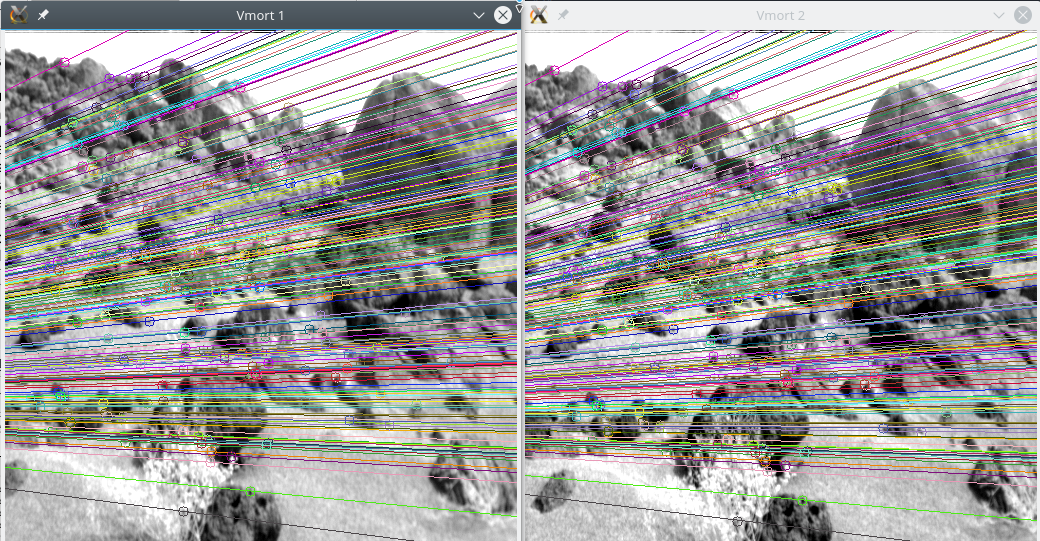
\includegraphics[width=0.7\textwidth]{Epipolares.png}}

    \section{Cálculo del movimiento de la cámara}

      Ahora debemos calcular los movimientos relativos de cada pareja de cámaras.
      Para ello se calculan los puntos en correspondencias igual que antes (en este caso se toma
      un umbral de $35$ para \emph{BRISK} para tomar más correspondencias),
      se calculan las matrices fundamentales entre cámaras (el orden es 1-2,2-3,1-3), las esenciales, y por último
      se aplica el algoritmo euclídeo de reconstrucción para reconstruir dichas matrices.

      \begin{lstlisting}
        // Euclidean reconstruction algorithm!
        for (unsigned i = 0; i < essentials.size(); i++)
        {
          cout << "Fundamental " << fundamentals[i] << "\n" << endl;
          Mat E = essentials[i];

          // Normalize
          Mat eet = E.t() * E;
          eet /= trace(eet).val[0] / 2;
          eet = Mat::eye(3,3,CV_64FC1) - eet;
          E /= sqrt(trace(eet).val[0] / 2);


          // Getting translation
          int max_row = 0;
          if(eet.at<double>(1,1) > eet.at<double>(0,0))
            max_row = 1;
          if(eet.at<double>(2,2) > eet.at<double>(max_row,max_row))
            max_row = 2;

          Vec3d T(eet.row(max_row));
          T /= sqrt(eet.at<double>(max_row,max_row));

          Mat R, R1, R2, R3;

          // For each point, recover Z_i and Z_d
          for (unsigned p = 0; p < corresp[i][0].size(); p++)
          {
            Point2d p_i = corresp[i][0][p];
            Point2d p_d = corresp[i][1][p];

            double x_d = p_d.x;

            double Z_i = -1.0, Z_d = 1.0;

            int i = 1;

            while ((Z_i <= 0.0 || Z_d <= 0.0) && i <= 4)
            {
              if ((Z_i < 0.0 && Z_d > 0.0) || (Z_i > 0.0 && Z_d < 0.0))
              {
                E = -E;

                // Get w
                Mat w[3];
                Mat tmp(T, CV_64FC1);
                tmp = tmp.t();

                w[0] = E.row(0).cross(tmp);
                w[1] = E.row(1).cross(tmp);
                w[2] = E.row(2).cross(tmp);

                R1 = w[0] + w[1].cross(w[2]);
                R2 = w[1] + w[2].cross(w[0]);
                R3 = w[2] + w[0].cross(w[1]);

                R = Mat(3,3, CV_64FC1);
                R1.copyTo(R.row(0));
                R2.copyTo(R.row(1));
                R3.copyTo(R.row(2));

                Mat p_hom = Mat(Vec3d(p_i.x, p_i.y, 1.0));
                Mat T_mat = Mat(T);

                // Get Z_i and Z_d
                Mat aux = (f_d * R1 - x_d*R3);

                Mat num = aux * T_mat;
                Mat den = aux * p_hom;

                Mat m_Z_i = f_i * num / den;

                Z_i = m_Z_i.at<double>(0,0);

                Mat pt_3D_i = Z_i * p_hom / f_i;

                Mat m_Z_d = R2 * (pt_3D_i - T_mat);
                Z_d = m_Z_d.at<double>(0,0);

              }

              if (Z_i < 0.0 && Z_d < 0.0)
              {
                T = -T;
                Mat p_hom = Mat(Vec3d(p_i.x, p_i.y, 1.0));
                Mat T_mat = Mat(T);

                // Get Z_i and Z_d
                Mat aux = (f_d * R1 - x_d*R3);

                Mat num = aux * T_mat;
                Mat den = aux * p_hom;

                Mat m_Z_i = f_i * num / den;

                Z_i = m_Z_i.at<double>(0,0);

                Mat pt_3D_i = Z_i * p_hom / f_i;

                Mat m_Z_d = R2 * (pt_3D_i - T_mat);
                Z_d = m_Z_d.at<double>(0,0);
              }
              i++;
            }

          }

          if (i >= 5)
          {
            cout << "Failed reconstruction!" << endl;
            return false;
          }

          Rt.push_back(pair<Mat,Vec3d>(R,T));
        }
      \end{lstlisting}

      En este caso los resultados no son buenos por algún error en la implementación,
      ya que la primera matriz de rotación sale rarísima, sus elementos son demasiado
      grandes. Las demás no tienen mala pinta.


\end{document}
